\chapter{Data}
The speed of light is approximately 299,792,458 meters per second, making it the fastest-known phenomenon in the universe. The speed of seismic waves is very low compared to light and that's why \textbf{earthquake comes} and \textbf{lightning strikes}.

Getting figure here- 

\begin{figure}[H]
    \centering
    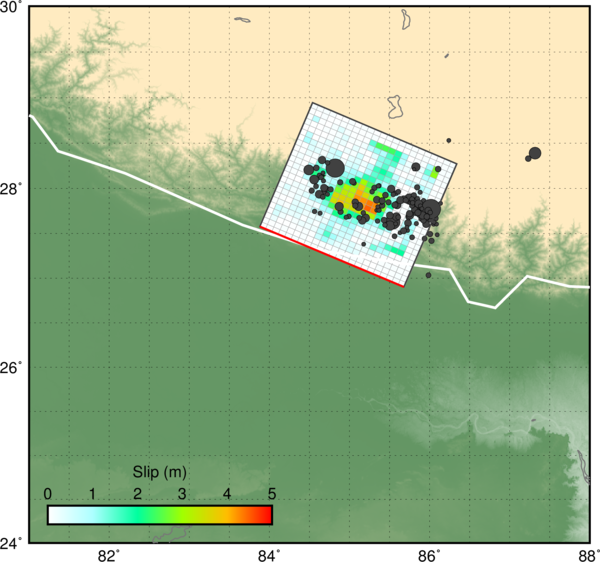
\includegraphics[width=\textwidth]{basemap.png}
    \caption{ Do caption your maps properly}
    \label{fig:well}
\end{figure}


\newpage
